
\section{Results}

Here, We have the result of quantitative measures to assess the level of agreement between the data and the simulation, using the GOF scores, which is discussed in details in evaluation method section. We begin by presenting the overall final result, and then break it down into some of its different components and combinations. 

Fig.~\ref{fig:gof} presents GOF results of all four vesions of velocity models for some selected events with largest number of stations. The countour surface in these plots are built based on FS values computed at each section. Although the spacial interpolation for colored surface is artificial, it is facilitate understaing of results and it is consitant with previous similar works. Brighter colors corresponds to higher scores and consequently better matchs. Fig.~\ref{fig:gof} also includes histograms of the scores in interval of 0.5 points on the 0 to 10 scoring scale. Having histograms with a tendency toward right side of the scale indicates more stations with higher scores. We can see an overall improvement in this matter, while going from CVM-S4 to CVM-S4.26.223.

\begin{figure*}
    \centering
    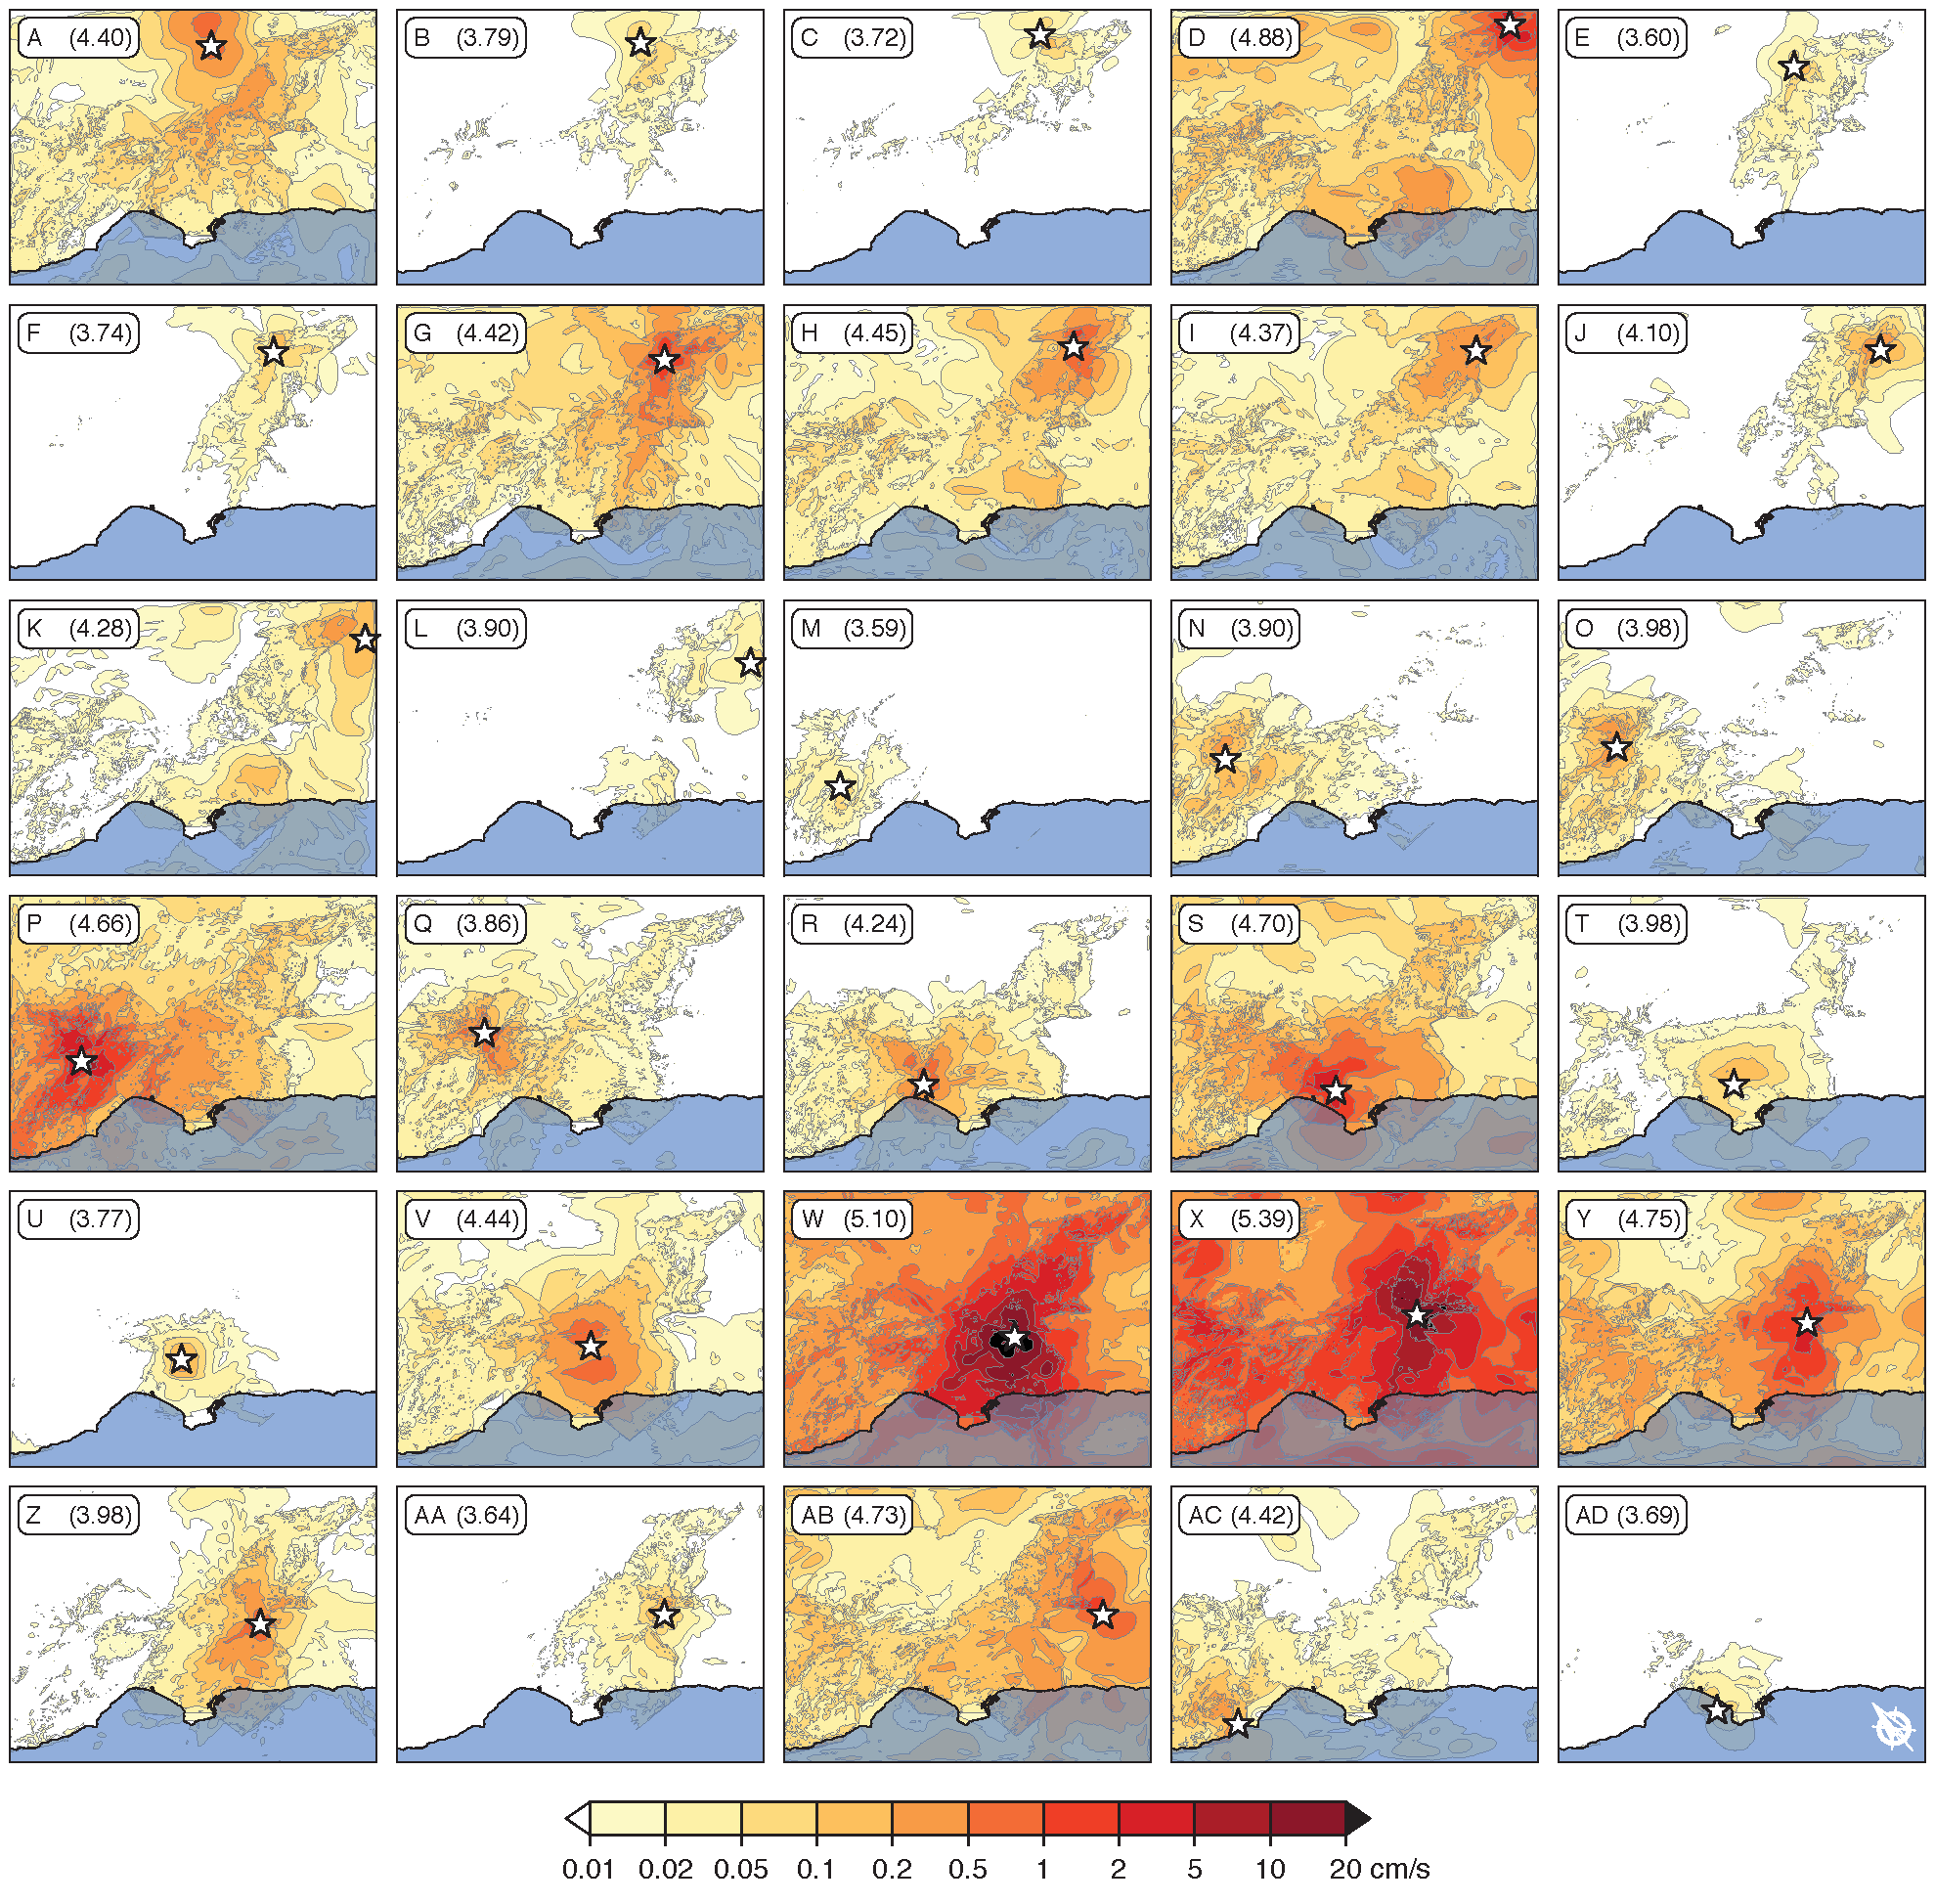
\includegraphics
 [width=\textwidth]
     	{figures/pdf/figure-03}
    \caption{GOF map for selected events with higher number of stations. Countours indicate the total FS score coming from the average of results in 3 directions. Event codes and their number of stations are mentioned in the plots.  . all the events comparing 3 versions of CVM-S4.26 with  CVM-S4 velocity model. Stations are depicted by dots and epicenters are located by stars. }
    \label{fig:gof}
\end{figure*}



Since the models differ only in detailes, the scores corresponding to them would be close and the difference plots can better highlight the differences and would be more helpful to discuss the results. Fig.~\ref{fig:gof_diff} shows differece between the distribution of total scores for all the validation stations in the region of interest for any of the events for 3 versions of CVM-S4.26 with respect to CVMS-4. This figure illustrates the wide range of results indicating events and areas in which any of the velocity models have better results. 


\begin{figure*}
    \centering
    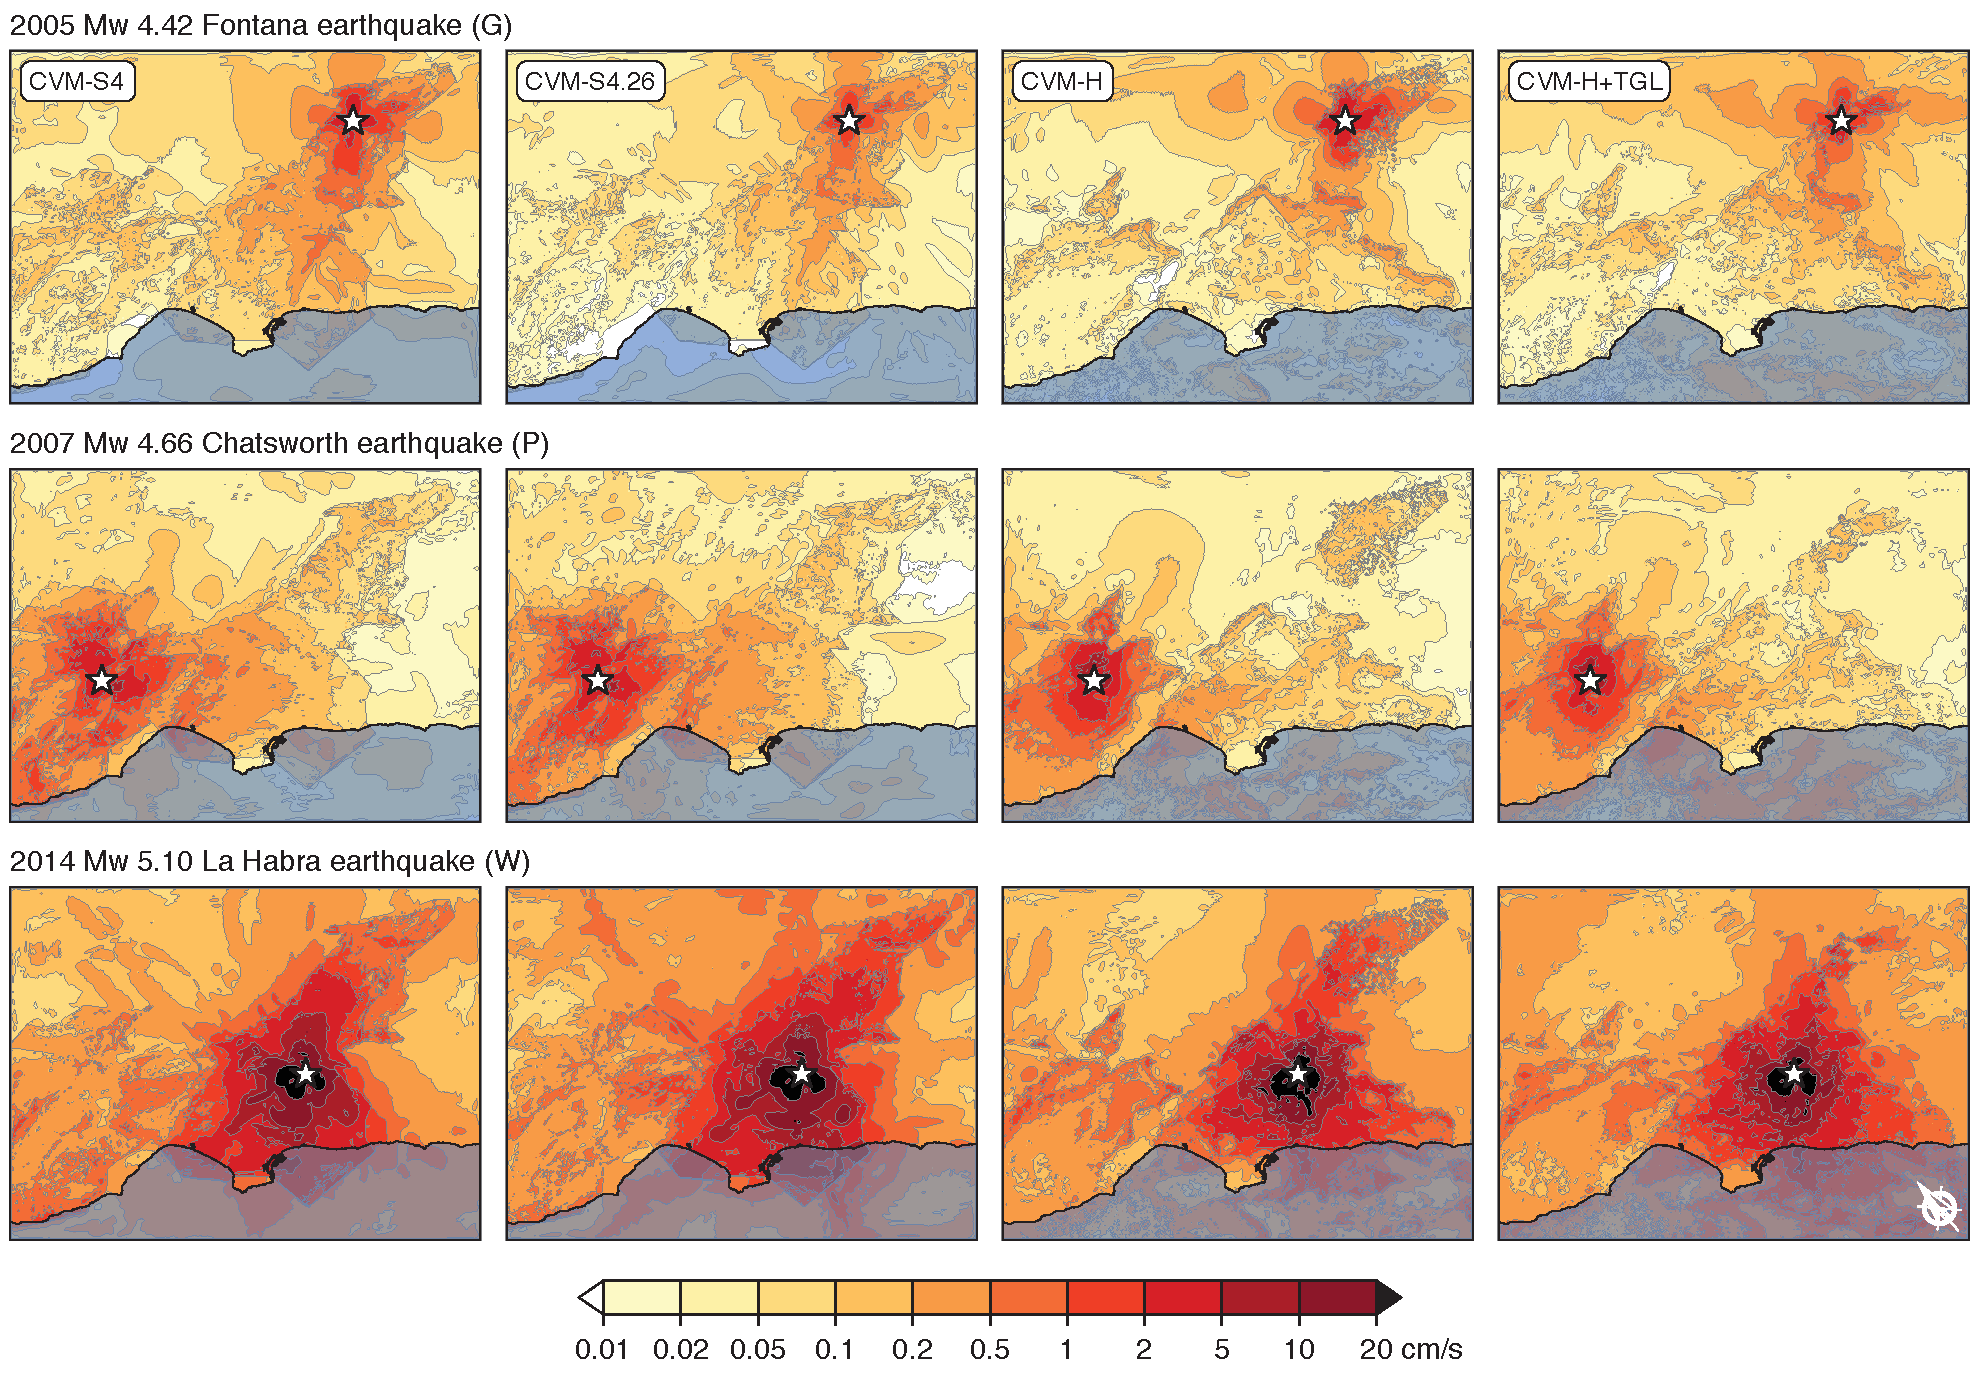
\includegraphics
 [width=0.75\textwidth]
     	{figures/pdf/figure-04}
    \caption{difference GOF map for all the events comparing 3 versions of CVM-S4.26 with CVM-S4 velocity model. Stations are depicted by dots and epicenters are located by stars. }
    \label{fig:gof_diff}
\end{figure*}


In the next step, we investigate the results of improvent in goodness of fit scores of 3 different versions of CVM-S4.26 with respect to original version, CVM-S4, for the broad band and in different defined band widths. The results are presented for 2008 Chino Hills Earthquake. There were studies previously for this events showing that simulations produced results closer to observations in the lower frequency bands for velocity model CVM-S4 \citep{Taborda_2013_BSSA}. Similar results were confirmed by \citet{Taborda_2016}for both models CVM-S4 and CVM-S4.26.223. Similar results can be noted for all different versions of CVM-S4.26. The overall improvement with respect to CVM-S4 model is more noticable at lower frequency band (0.1-0.25~Hz) than in higher frequncy bands. 

\begin{figure*}
    \centering
    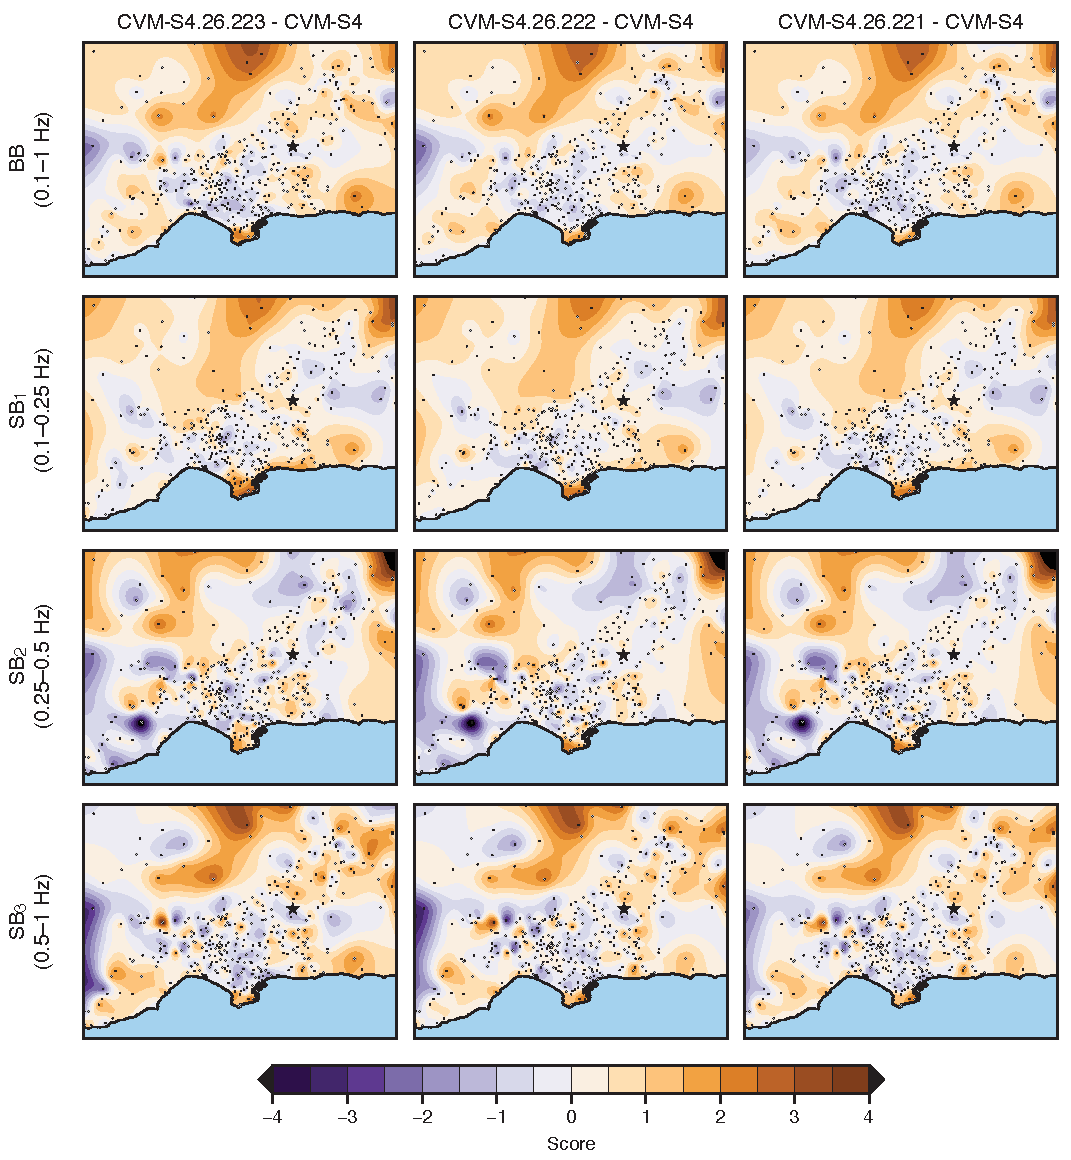
\includegraphics
 [width=\textwidth]
     	{figures/pdf/figure-05}
    \caption{Improvement GOF map Chino Hills earthquake for broad band and for different bandwidths. Stations are depicted by dots and epicenters are located by stars. }
    \label{fig:bands}
\end{figure*}